\documentclass[conference]{IEEEtran}
\usepackage{graphicx}
\usepackage{amsfonts}
\usepackage{amssymb}
\usepackage[spanish]{babel}
\usepackage{verbatim}
\usepackage{amsbsy}
\usepackage{algorithm}
\usepackage{algorithmic}
\usepackage[T1]{fontenc}		%Previene errores en el encoding
\usepackage[utf8]{inputenc}		%para identificar acentos(encoding)
\usepackage{hyperref} %para url´s 
% correct bad hyphenation here
\usepackage{placeins} %para el FloatBarrier
\hyphenation{optical networks semiconductor IEEEtran}
\decimalpoint %decimales
\newtheorem{definition}{Definicion}[section]
\newtheorem{theorem}{Teorema}[section]
\newtheorem{lemma}{Lema}[section]

\begin{document}

% paper title
\title{Segmentación de imágenes de células con cáncer, utilizando el algoritmo Normalized Cut\\ \small (Un conjunto de enfoques y ensayos).   }


% author names and affiliations
% use a multiple column layout for up to three different
% affiliations
\author{\IEEEauthorblockN{García Ramírez, J. Antonio \small{jose.ramirez@cimat.mx}}
\IEEEauthorblockN{Mendez Ramírez, Kenny Yahir \small{kenny.mendez@cimat.mx}} 
\IEEEauthorblockA{Centro de Investigacion en Matematicas. Unidad Monterrey\\
}
}



% make the title area
\maketitle

\begin{abstract}
%Desde hace años existe una brecha entre el cálculo con matrices en gran escala y el \textit{big data}, 
En este trabajo aplicamos el algoritmo de Normaliced Cut para segmentar imágenes de células con cáncer. En vista de que el ambiente R \cite{R} posee pocas herramientas para analizar imágenes, en este trabajo compartimos una implementación del algoritmo Normalized Cut en el mismo con extensiones a programas y procesos realizados en C++, para proveer al usuario una amigable interfaz en R para segmentar imágenes. A la par se discuten y comentan los resultados obtenidos al considerar diversos enfoques para atacar la impracticidad del algoritmo Normalized Cut en gran escala. 

\textit{Key words: Normaliced Cut, segmentación de imagenes, algoritmo de Lanczos, valores y vectores propios, grafo, matriz de similaridad, R, kernels y gran escala.
}\end{abstract}

\IEEEpeerreviewmaketitle


\section{Introducción y motivación}
El reconocimiento estadistico de patrones, y en particular el analisis de imágenes, es un estimulante campo de estudio donde conviven la estadistica y las ciencias de la computación. En los años recientes el ambiente de computo estadistico y lenguaje de programación R \cite{R} ha aumentado su presencia en el análisis estadístico e inclusive es utilizado en contextos de cómputo en la nube y big data, por otro lado, el análisis de imágenes es un área que sigue motivando investigación.\\

En contrapunto de lo esperado, pues el análisis de imágenes emplea diferentes técnicas de aprendizaje estadístico (tanto supervisado como no supervizado), el ambiente R posee pocas herramientas para análisis de imágenes como se puede comprobar al revisar la entrada de ‘MedicalImaging’ de su Task View,  frente a otras herramientas especializadas como OpenCV \cite{OpenCV}. Por su parte existen entornos de computo científico que integran algunas herramientas para analizar imágenes, pero sus capacidades se ven reflejadas en su precio comercial, por ejemplo MatLab \cite{MatLab}. \\

Lo anterior aunado al hecho de que la segmentación de imágenes es un objetivo final y a veces solo un paso intermedio en otras investigaciones, en el presente trabajo se comparte una aplicación de segmentación de imágenes de células con cáncer 
utilizando el algoritmo Normalized Cut, al cual nos referiremos en lo siguiente como \textit{Ncut}. Con el fin de proveer a los usuarios y desarrolladores del lenguaje R de una implantación del algoritmo Ncut (la cual no existe en OpenCV y otros entornos de computo científico). \\
Previamente se trabajó en la codificación de dos programas\footnote{Vease \url{https://www.overleaf.com/read/pnqsbjrmyhvk} para más detalles sobre la implementación en su sección III} de lo cual se parte como base para comparar los resultados parciales de diferentes enfoques al implementar el algoritmo de \textit{Ncut} para segmentar imágenes de células con cáncer en la sección III de este trabajo, por su parte la sección II solo contempla una breve reseña sobre la teoría y puntos a considerar en la aplicación e implementación del método \textit{Ncut}. Los resultados parciales y poco alentadores se presentan en la sección IV para concluir en la sección V con una evaluación del enfoque actual y los caminos recorridos además de detallar posibles futuros trabajos en la implementación de \textit{Ncut} en mediana y gran escala.\\



\section{Reseña sobre el algoritmo \textit{Ncut}}

\subsection{Sobre el problema de segmentar de imágenes y el enfoque de \textit{Ncut}}

El problema de segmentar una imagen (considerando los valores que puede tener cada pixel en diferentes canales) se suele formular en términos matemáticos de la siguiente manera: dada una imagen cuyo conjunto de pixeles $V$, se busca particionar $V$ en conjuntos disjuntos $V_1,V_2, \dots,V_m$ donde alguna medida de similaridad (es decir de parecido) entre los pixeles de cada $V_i$ es alta, mientras la misma medida a través de conjuntos diferentes $V_i$, $V_j$ es baja.\\

Si bien la anterior medida de similaridad responde a la importancia de percepciones visuales, espaciales y de agrupación ésta debe de ser compartida en pixeles próximos. En vista de que el conjunto de todas las posibles particiones de un conjunto $V$ crece exponencialmente como función de la cardinalidad de $V$\footnote{De hecho, esta es la definición de los números de Stirling del segundo tipo.}, surge la pregunta ¿Cómo escoger la partición \textit{correcta}?\\

De manera general existen dos maneras de abordar el problema anterior: el primero consiste en prestar atención a niveles bajos de coherencia entre brillo, color y textura en cada pixel, sin embargo éste enfoque tiende a producir segmentaciones jerárquicas donde las jerarquías mayores responden a grupos y las menores a pixeles individuales, esto en la practica puede efectuarse con algoritmos computacionalmente costosos como los populares ‘single’ y ‘ward’ que producen dendogramas.\\

En contraste, el segundo enfoque para abordar el problema es el que comparte \textit{Ncut}, el cual es un enfoque \textit{hacia abajo} es decir que primero presta atención en áreas y rasgos de mayor tamaño y luego presta atención a los detalles, siguiendo la analogía de \cite{Ncut} ''como un pintor primero marca las áreas grandes y después llena los detalles''.\\

Siguiendo las ideas de \cite{Ncut}, el problema de la segmentación de imágenes consiste en dos puntos: \\
\begin{enumerate}
\item ¿Cuál es el criterio preciso para una buena partición?, es decir definir la similaridad entre elementos de $V$. 
\item ¿Cómo puede tal partición ser calculada eficientemente?\\
\end{enumerate}  

De manera breve, el enfoque sugerido por \cite{Ncut}, para particionar una imagen consiste en considerar a los pixeles de una imagen $V$ como los vértices de una grafica $G=(V,E)$ y formar una partición en dos conjuntos $A$ y $B$ tales que $A \cup B = V$, $A \cap B = \emptyset $, simplemente removiendo aristas que conecten ambas partes. El grado de disimilaridad entre $A$ y $B$ puede calcularse como el peso total de las aristas que fueron removidas, en teoria de grafos esto es llamado \textit{corte}:
\[
cut(A,B) = \sum_{u\in A, v\in B} w(u,v)
\]
Encontrar el corte mínimo es un problema bien estudiado y existen algoritmos eficientes para resolverlo. \\

Por otro lado \cite{Ncut} propone la siguiente medida de disociación entre grupos, el \textit{normalized cut}, que posee la ventaja de considerar particiones con mayor número de elementos, pues la medida de disimilaridad se encarga de excluir los casos en donde el \textit{corte} proporciona particiones con un solo elemento en una partición:
\[
Ncut(A,B)= \frac{cut(A,B)}{assoc(A,V)}+\frac{cut(A,B)}{assoc(B,V)}
\]
Donde $assoc(A, V) = \sum_{u\in A,t\in V}w(u,t)$ corresponde con el total de las conexiones de los nodos del conjunto $A$ a todos los nodos del grafo y $assoc(B,V)$ es definido de manera similar. Un resultado fundamental de \cite{Ncut} es que minimizar la disociación a través de grupos, es decir la medida $Ncut$, es equivalente a maximizar la asociación dentro de cada grupo y que ambas condiciones pueden satisfacerse simultáneamente.   


\subsection{Aspectos matemáticos y computacionales}

Como es comentado en \cite{Ncut} encontrar el $Ncut$ óptimo exactamente es un problema NP-completo (cuya elegante prueba se encuentra en el apéndice A del mismo paper y es atribuida a Papadimitrou). Sin embargo, los mismos autores prueban que al relajar las condiciones al dominio continuo una solución aproximada al problema discreto puede encontrarse eficientemente y después de definir notación y con un poco de álgebra se muestra que esta solución aproximada a la minimización de $Ncut$ corresponde a:
\begin{equation}
\min_{\boldsymbol{x}} \textit{Ncut} (\boldsymbol{x}) = \min_{\boldsymbol{y}} \frac{\boldsymbol{y}^t(D-W)\boldsymbol{y}}{\boldsymbol{y}^tD\boldsymbol{y}}
\end{equation}
Donde $ \boldsymbol{x}$ es un vector indicador con 1 en la i-ésima posición si el i-ésimo pixel se encuentra en $A$ y -1 en todas las otras $|V|-1$ entradas, $D=diag(d_1,d_2,…,d_{|V|})$ es la matriz diagonal donde $d_i=\sum_j w(i,j)$, $W$ es simplemente la matriz de pesos de las aristas es decir $W (i,j)=w_{ij}$, y finalmente $ \boldsymbol{y}$ es el vector donde cada entrada $i\in \{1,-b\}$ con $b = \frac{\sum_{x_i>0}d_i}{\sum_{x_i<0}d_i}$ y $ \boldsymbol{y}D \boldsymbol{1} = 0$ donde $ \boldsymbol{1}$ es un vector de dimensión $|V|$ con 1’s en todas sus entradas. \\

De lo anterior los autores de \cite{Ncut} reconocen que (1) corresponde con el cociente de Rayleigh \cite{MatrixC}. Relajando la condición de que $\boldsymbol{y}$
 tome valores reales, se obtiene que (1) es minimizado por resolver el problema de valores propios generalizado:
\begin{equation}
(D-W)y = \lambda D y
\end{equation}
Como ellos lo demuestran, la ecuación (2) es equivalente al problema estándar de valores propios 
\begin{equation}
D^{-1/2}(D-W)D^{-1/2}z = \lambda z\label{eq:laplacian_mat}
\end{equation}
Donde $z=D^{1/2} y$. Una propiedad interesante de (3) es que $z_0= D^{1/2} \boldsymbol{1}$ es un vector propio asociado al valor propio 0, más aun $ D^{-1/2}(D-W)D^{-1/2}$ es simétrica y semi definida positiva (más adelante nos referiremos a esta matriz como $L$), por lo que $z_0$ es el vector propio asociado al valor propio más pequeño y por el resultado espectral conocido de cursos de álgebra lineal, los vectores propios de una matriz son perpendiculares entonces el vector propio asociado al segundo valor propio más pequeño de (3) es perpendicular a $z_0$. Entonces el vector propio asociado al segundo valor propio más pequeño de (3) es la solución real de (2). \\

En todo nuestro conjunto de enfoques y ensayos se utiliza explícitamente (3) para encontrar la partición deseada por medio de los valores y vectores propios correspondientes.\\

Como se expone en \cite{Ncut} existen varias peculiaridades sobre el uso del resultado anterior. Por un lado una imagen se puede segmentar utilizando los $k$ valores propios más pequeños, y sus correspondientes vectores propios, lo cual es computacionalmente costoso por las dimensiones de $W$ pues si la imagen original es de tamaño $h \times w$ entonces $W$ tiene dimensiones $(h\times w)\times (h\times w)$.\\

Por otro lado se puede partir de encontrar la primer solución de (3) y realizar el mismo procedimiento sobre cada conjunto $A$ y $B$ (lo cual es computacionalmente más eficiente, pues previamente ya se calculo la matriz $W$ sin embargo esto es impráctico pues involucra almacenar en memoria a la matriz $W$ completa). \\

Nuestro enfoque consistió en segmentar utilizando el vector propio asociado al segundo valor propio más pequeño de (3) para identificar dos grupos. Es importante mencionar que en vista de la naturaleza del algoritmo $Ncut$ la fase de preprocesamiento de las imágenes con las que se trabajó no contempla ningún filtro sobre la imagen original.   \\

Entonces el algoritmo de agrupación empleado en nuestras aplicaciones consiste en:\\
\begin{enumerate}
\item Dada una imagen de tamaño $h \times w$ con $n$ canales, considerada como un grafo $G=(V,E)$, construir la matriz de pesos $W$ (en algunos casos se consideró almacenar el cálculo de esta matriz en memoria y en otros escenarios la matriz se recalcula en cada iteración con la finalidad de no almacenarla) conectando dos nodos con una medida de similaridad. Para lo cual elegimos un kernel gaussiano definido como 
\[
W_{ij}= e^{-||x_{(i)}-x_{(j)}||^2_2/2\sigma^2_I}e^{-||x_{(i)}-x_{(j)}||^2_2/2\sigma_x^2}
\] 
Si $||x_{(i)}-x_{(j)}||_2^2 < r^2$ y 0 en otro caso. Donde $x_{(i)}$ es el i-ésimo pixel de la imagen. En nuestros experimentos fijamos $\sigma_x^2=10$, $\sigma_I^2=0.05$ y siguiendo la recomendación de \cite{Ncut} fijamos $r = \left \lfloor
 \sqrt{\frac{(h\times w)-1}{2}*0.1}\right \rfloor +1 $, es decir que consideramos que cada pixel se conecta a lo más con $r^2$ pixeles alrededor de él usando la métrica $L_2$.\\  

\item Resolver (3) y guardar él vector propio asociado al segundo valor propio más pequeño. \\

\item Usar el vector propio asociado al segundo valor propio más pequeño y aplicar sobre sus entradas una sencilla regla de separación la cual consiste en asignar a cada píxel la partición '+1' si su correspondiente entrada en el segundo vector propio es positiva y '-1' en caso contrario.
\end{enumerate}
De manera general resolver el problema de valores propios para todos los valores requiere de $O(p^3)$ operaciones, donde $p$ es el número de pixeles de la imagen (en nuestra notación $p = h \times w$), lo cual hace impráctico $Ncut$ para segmentación de imágenes grandes, sin embargo en nuestros experimentos logramos manejar imágenes hasta con 11,280 pixeles ($120 \times 90$).\\

Pero para nuestra aplicación en particular tenemos aspectos que favorecen el cómputo: primero nuestra matriz $W$ es simétrica (lo cual es consecuencia de la simetría del kernel usado) , semidefinida positiva y esparcida (en vista de la construcción de $r$) y solo requerimos de un par de los valores propios más pequeños, como se menciona en \cite{Ncut} la precisión de los valores propios es baja pues como pudimos comprobar de manera experimental la distribución da las entradas de los vectores propios mencionados deja claro que con solo saber el signo correspondiente a la entrada del vector propio basta para clasificar y en adición a los comentarios de \cite{Ncut}  experimentalmente encontramos que el calculo de $W$ solo requiere de operaciones entre números de aritmética flotante del tipo \textit{float} en C++ en una arquitectura de 64bits. Las propiedades antes mencionadas son totalmente explotadas por el método de Lanczos, el cual tiene una complejidad de $O(mp)+O(mM(p))$ \cite{MatrixC} donde $m$ es el máximo número de cálculos del tipo matriz-vector (con matrices esparcidas) y $M(p)$ es el costo de la multiplicación de matriz-vector, como se trabaja con matrices esparcidas la complejidad de $M(p)$ es $O(p)$.

\section{Enfoques de implementación propuestos}

\subsection{Implementación base en el entorno de programación R}

En este primer enfoque se partió de la trabajada anteriormente implementación de \textit{Ncut} en el ambiente de programación R\footnote{El código puede consultarse en \url{https://github.com/fou-foo/MCE/tree/master/Second/Numerico/ProyectoFinal} en los archivos ‘mini\_Ncut\_RGB\_float.R’ y ‘W\_RGB\_float.cpp’ que aceptan como entrada la imagen localizada en el archivo ‘001.jpg’.}, los resultados para una sola imagen de células con cáncer se presentan en la siguiente sección.\\

En este enfoque el flujo de trabajo que se siguió para segmentar imágenes usando \textit{Ncut} se muestra en la figura 1 donde el color azul indica que en esa tarea se ejecutó empleando el lenguaje R y el color naranja indica que la tarea se realizó por medio del lenguaje C++. En particular el preprocesamiento del segundo paso consistió en cortar la imagen original (de tamaño $3,000 \times 2,239$ pixeles) en 600 imágenes más pequeñas (de medidas $120 \times 90$) y realizar segmentación en dos grupos en cada una de estas 600 nuevas imágenes, en este enfoque se sacrifica información que se pierde al considerar segmentaciones locales (una por cada nueva imagen producida) en vías de lograr un resultado base con el cual contrastar los demás enfoques. Además la etapa de preprocesamiento consiste en normalizar los valores de los píxeles en cada canal para la imagen en sus dimensiones originales, es decir que en cada canal a cada valor de píxel se le restó el valor mínimo encontrado en el canal y se dividió el resultado entre el rango del canal original (diferencia entre el valor máximo y el mínimo) con la finalidad de aumentar el contraste en toda la imagen y mantener una propiedad global en todas las 600 imágenes más pequeñas sobre las que se segmenta.\\

\begin{figure}[htbp]
\center{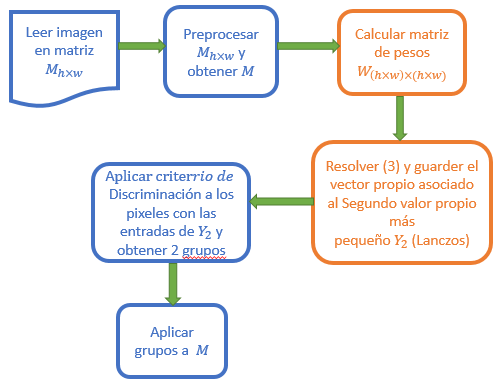
\includegraphics[width=7cm]{workflow1.png}}
\caption{Flujo de trabajo base para segmentar imágenes}
\label{workflow}
\end{figure}

El lenguaje de programación R, al igual que otros lenguajes no compilados, en particular posee retos en la aplicación del algoritmo \textit{Ncut} debido a las siguientes razones: 
\begin{enumerate}
\item La representación de las imágenes y en general de los números de punto flotante corresponden al estándar de \textit{double} del lenguaje C++
\item Carga en memoria RAM todos los objetos con los que se trabaja. 
\end{enumerate}
Sin embargo las matrices esparcidas son fáciles de manejar en el ambiente R.\\

Para contrarrestar el primer punto anterior el cálculo de la matriz $W$ (en cada una de las 600 imágenes más pequeñas) se realiza en C++ restringiendo el tipo de dato entre operaciones al tipo \textit{float}, para lo cual se emplea el paquete Rcpp \cite{Rcpp} y para almacenar la matrices en un formato de matriz esparcida se emplea el paquete RcppEigen \cite{RcppEigen} el cual permite interactuar con la librería Eigen del lenguaje C++, de manera que la salida del código C++ es una matriz $W^*$ simétrica, semidefinida positiva y del tipo esparcida que incorpora la información necesaria para resolver el problema de valores propios de la ecuación (3).\\ 

Hasta este punto utilizar el lenguaje C++ para el cálculo de $W$ mejoro notoriamente el tiempo de ejecución en comparación de hacerlo en R nato, además se ahorró espacio en memoria del 50\% al usar solo el tipo de dato \textit{float} en lugar de \textit{double}. \\

Para contrarrestar el segundo punto de la lista anterior se remueven constantemente del ambiente de manera explícita los objetos que ya no se requieran y haciendo llamado explicito al \textit{garbage collector} de R así para el cuarto paso se emplea una función de la librería Rspectra \cite{RSpectra}, que es una interfaz a la librería Spectra desarrollada en C++ similar a la librería ARPACK\cite{Arpack} (desarrollada en Fortran) , que hace referencia a una implementación en C++ del método de Lanczos reiniciado implícitamente y para obtener los valores propios más pequeños en lugar de los más grandes (que son la salida del método de Lanczos) se utiliza el método de shift alrededor del cero en lugar de invertir explícitamente la matriz $W^*$.\\

En este enfoque simplificado, hecho que se implementa en el quinto paso de la figura 1, se supone que de manera a priori se podrán distinguir solo dos grupos, el formado por los píxeles cuya presencia se encuentra en el grupo etiquetado como ‘-1’ si en alguna de las 600 segmentaciones sobre imágenes más pequeñas su correspondiente entrada del vector propio asociado al segundo valor propio más pequeño es negativa y ‘+1’ en el otro caso.

\subsection{Enfoque utilizando paralelismo implícito.}
En vista de que el enfoque utilizado en la sección anterior tiene une dos puntos débiles: el primero que requiere de almacenar completamente en memoria principal o secundaria toda la matriz de pesos $W$ y el segundo es que es una implementación lineal. Para contrarrestar el almacenamiento de la matriz $W$ se consideró realizar una implementación propia del método de Lanczos reiniciado implícitamente (así se sacaría provecho de la naturaleza esparcida de la ecuación (3)) que tuviese como entrada una imagen y como salida la matriz tridiagonal y los vectores propios asociados a los valores propios más pequeños de la matriz que determina (3).\\

En un primer intento se consideró emplear un framework como PyTorch \cite{PyTorch} para agilizar el desarrollo de la implementación, sin embargo se descubrió que para lograr la implementación mencionada se requiere de un enfoque de paralelismo explícito como CUDA, en donde se pueda asignar a hilos individuales posiciones de la imagen y que en caso de no cumplir con las restricciones que impone el parámetro $r$ (de la construcción de $W$) el hilo muera rápidamente. Así es como vemos a un esquema de paralelismo explícito y a la fuerte teoría que respalda la convergencia de diversas implementaciones del método de Lanczos \cite{MatrixC} como una posible solución al problema de almacenamiento de $W$.


\subsection{Segmentación usando los vectores propios de $W^{-1}$ con \texttt{MLlib}}


Como se observa en la Figura \ref{flowchart_invert_laplacian}, el otro enfoque usando la librería \texttt{MLlib} en Apache Spark con el lenguaje \texttt{Scala}, podemos recurrir a un cojunto de métodos básicos de álgebra lineal para obtener los valores propios (y sus vectores asociados) más pequeños de la matriz definida en (\ref{eq:laplacian_mat}). Entonces con el tipo de objeto \texttt{RowMatrix} y los métodos como \texttt{qr()}, \texttt{computeSVD()}, en teoría podemos calcular dichos valores y vectores asociados, los cuales ocuparemos como entrada para \texttt{kmeans} en el enfoque base.

\medskip

De esto se hicieron pequeñas pruebas mediante la máquina virtual de Cloudera Quickstart 5.13.0-0 en el ambiente de Hadoop de un solo nodo en una máquina con procesador Intel Core i7-6700HQ con una velocidad de 2.60 Hz octa core. Con éxito se pudieron calcular los primeros 20 valores y vectores propios de la matriz de pesos $W$. Esta matriz de pesos, como se ilustra en el diagrama de la Figura \ref{flowchart_invert_laplacian}, es calculada previamente con código en lenguaje \texttt{C}, escrita a un archivo de texto en formato \textit{RowMatrix}, posteriormente es almacenada y distribuida en el sistema de archivos HDFS de Hadoop.

\begin{figure}[htbp]
\center{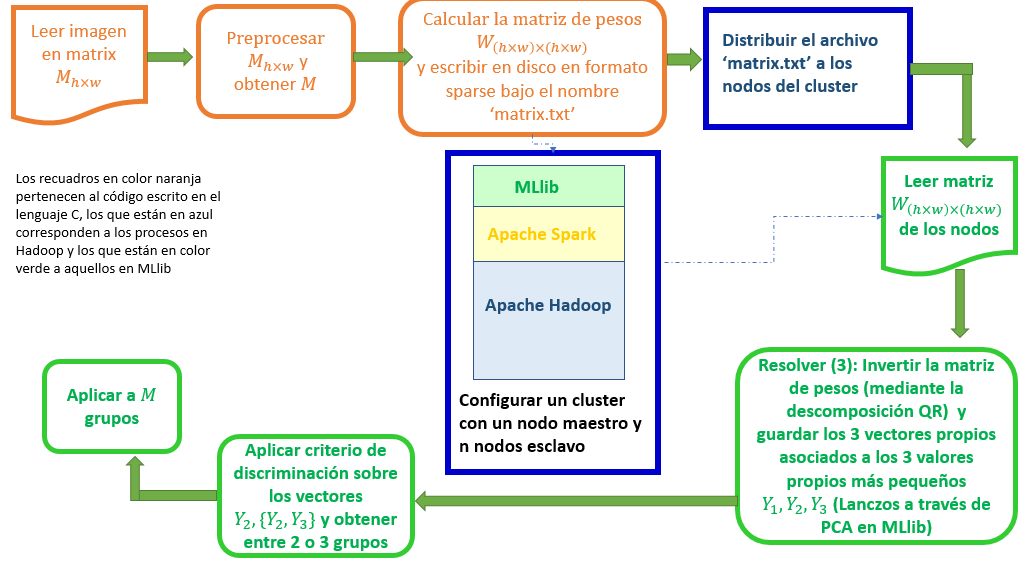
\includegraphics[width=8cm]{flowchart_qr_svd}}
\caption{Proceso de segmentación usando \texttt{MLlib}, se invierte la matriz construida en \ref{eq:laplacian_mat} y después se calculan sus valores propios más grandes.}
\label{flowchart_invert_laplacian}
\end{figure}

\subsection{Segmentación a través de Power Iteration Clustering con MLlib}

Dada la complejidad del planteamiento original y los demandantes requisitos para la implementación del Algoritmo \textit{Ncut}, exploramos más posibilidades además de las tecnologías ya disponibles como en el apartado anterior. Entre ellas encontramos, mas que otra tecnología o lenguaje, un algoritmo que trata de abatir este mismo tipo de problemas. Se trata del algoritmo \textit{Power Iteration Clustering}, basado en el método de potencias para el problema de valores y vectores propios \cite{PILin2010}. Actualmente está disponible mediante la librería \texttt{MLlib} en Apache Spark. La entrada del algoritmo requiere de haber procesado la matriz de pesos $W$ como en el enfoque inicial, y partir de ahí, definir el número de \textit{clusters} a identificar, el número de iteraciones a realizar y establecer la opción que normaliza el grado de los vértices (filas de $W$, para el caso de \textit{Ncut}).

\medskip

Aunque con la disposición de Hadoop y Apache Spark (\texttt{MLlib}) a través de la Máquina Virtual de Cloudera Quickstart 5.13.0-0 se pensó en realizar algunas pruebas para la segmentación de las imágenes de los ejemplos anteriores, no se pudo concretar debido a problemas técnicos de la propia ejecución del método \texttt{PowerIterationClustering()}. Sin embargo acorde al flujo de la Figura \ref{flowchart_pi1} podemos ver que este paso ya nos daba la segmentación final buscada (obtenemos la lista del etiquetamiento), aún para cuando se desearan encontrar más de 2 particiones.


\begin{figure}[htbp]
\center{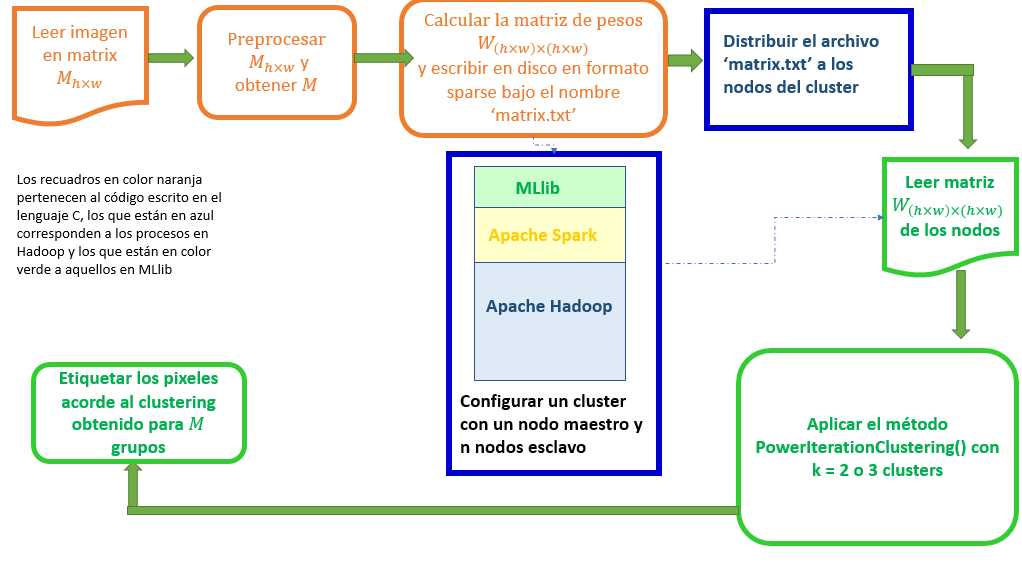
\includegraphics[width=8cm]{flowchart_pi}}
\caption{Proceso de segmentación usando el algoritmo \textit{Power Iteration} con Apache Spark. A diferencia de las otras alternativas, ésta detalla un flujo de trabajo más corto.}
\label{flowchart_pi1}
\end{figure}

\newpage
\section{Resultados}
Como ya se mencionó en el enfoque que hemos llamado base la imagen original se reescaló y posteriormente se dividió en 600 imágenes más pequeñas. Mostramos en la figura 4 el resultado de aplicar la actual implementación sobre la imagen ‘001.png’ de dimensiones $3,000 \times 2,239$ pixeles en 600 segmentaciones más pequeñas (de tamaños $120 \times 90$ píxeles) e independientes una de otra segmentación. Esta implementación es secuencial y actualmente requiere de aproximadamente 25 hrs de cómputo para una segmentación como la mostrada en la imagen 4 con un procesador Intel Core i7-7700HQ a una velocidad de 2.5GZ.\\

Como se puede apreciar en la siguiente imagen los resultados son desalentadores, pues pese al enorme tiempo de ejecución que requiere la implementación base, pues el supuesto de independencia en la segmentación de las imágenes es crucial. La independencia entre la segmentación de una subimagen y otra presenta diversos problemas como que aunque el tejido se diferencia del fondo de la imagen de manera global en ocasiones la etiqueta del grupo se pierde y el mismo tejido (sin hablar de la diferencia entre células con cáncer y células sin la enfermedad) es etiquetado como ‘-1’ o ‘+1’ en diversas segmentaciones. El resultado optimista es que el tejido es identificable lo que podría cuando menos comenzar a reducir la dimensionalidad del problema original al utilizar algoritmos como \textit{Power Iteration Clustering} cuya complejidad en tiempo y espacio depende del número de particiones a identificar.

\begin{figure}[htbp]
\center{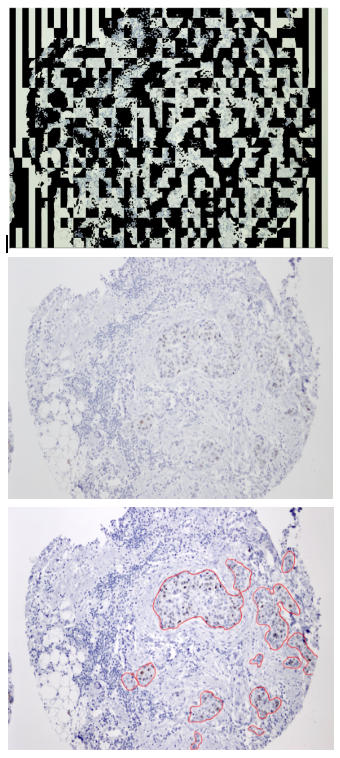
\includegraphics[width=7cm]{imagen_resultado_base.png}}
\caption{Resultado obtenido con la segmentación inocente del enfoque llamado base. Segmentación obtenida sobre las 600 sub-imágenes (arriba), imagen original (en medio) resultado deseado (abajo).}
\label{res_base}
\end{figure}
\FloatBarrier






\section{Conclusiones}
De manera general lo aprendido en el presente trabajo es que el algoritmo de \textit{Ncut} presenta serios problemas de escalamiento a pesar de su potencial para segmentar imágenes como se mostró en un trabajo anterior a este.\\

En analogía de otros muchos métodos de clasificación espectrales y basados en kernels, como \textit{string-kernels} o \textit{kernel PCA}, el algoritmo \textit{Ncut} requiere de seleccionar apropiadamente un kernel (en este caso la función que utilizamos para construir la matriz de similaridad $W$ hecho que puede favorecer a un enfoque de paralelismo explícito).\\

En contrapunto a los métodos mencionados \textit{Ncut} posee una \textbf{elegante} formulación que combina resultados básicos de álgebra lineal y teoría de grafos, que lo hacen atractivo y \textit{nos anima a trabajos posteriores} donde se requiera de conocimientos avanzados de paralelismo o bien un mayor emprendimiento de tecnologías como \cite{Hadoop} y \cite{MatrixSpark}.


\begin{thebibliography}{1}


\bibitem{MatrixSpark}
Bosagh Zadeh, Reza and Meng, Xiangrui and Ulanov, Alexander and Yavuz, Burak and Pu, Li and Venkataraman, Shivaram and Sparks, Evan and Staple, Aaron and Zaharia, Matei; \textit{Matrix Computations and Optimization in Apache Spark}, Proceedings of the 22Nd ACM SIGKDD International Conference on Knowledge Discovery and Data Mining, KDD '16 2016, ISBN:978-1-4503-4232-2; San Francisco, California, USA; pags 31--38,
\url{http://doi.acm.org/10.1145/2939672.2939675}



\bibitem{OpenCV}
Bradski, G., \emph{The OpenCV Library}, journal Dr. Dobb's Journal of Software Tools id:2236121, 2008-01-15, year 2000 


\bibitem{Rcpp}
Dirk Eddelbuettel and James Joseph Balamuta (2017). \emph{Extending R with C++: A Brief Introduction to Rcpp}. PeerJ Preprints 5:e3188v1, \url{https://doi.org/10.7287/peerj.preprints.3188v1.}

\bibitem{RcppArmadillo}
Dirk Eddelbuettel, Conrad Sanderson (2014), \emph{RcppArmadillo: Accelerating R with high-performance C++ linear algebra}, Computational Statistics and Data Analysis, Volume 71, March 2014, pages 1054-1063. \url{  http://dx.doi.org/10.1016/j.csda.2013.02.005}

\bibitem{RcppEigen}
Douglas Bates, Dirk Eddelbuettel (2013), \emph{Fast and Elegant Numerical Linear Algebra Using the RcppEigen Package}, Journal of Statistical Software, 52(5), 1-24. \url{http://www.jstatsoft.org/v52/i05/}


\bibitem{MatrixC}
G.H. Golub and C.F. Van Loan, \emph{Matrix Computations}, John
Hopkins Press, 1989.

\bibitem{PyTorch}
PyTorch core team (2018), \emph{Tensors and Dynamic neural networks in Python with strong GPU acceleration.},  \url{https://pytorch.org/}


\bibitem{R}
R Core Team, \emph{R: A Language and Environment for Statistical Computing}, R Foundation for Statistical Computing; Vienna, Austria, 2014 y  \url{http://www.R-project.org/}

\bibitem{Arpack}
Richard B Lehoucq, Danny C Sorensen, and Chao Yang, \textit{ARPACK users' guide: solution of large-scale eigenvalue problems with implicitly restarted Arnoldi methods}, volume 6. Siam, 1998.


\bibitem{imager}
Simon Barthelme (2017). \emph{imager: Image Processing
  Library Based on 'CImg'}, R package versión  0.40.2., \url{  https://CRAN.R-project.org/package=imager}


\bibitem{Ncut}
Shi J. and Malik J., \emph{Normalized Cuts and Image Segmentation}, IEEE Transactions on pattern analysis and machine learning, VOL. 22, No. 8, Agosto 2000.


\bibitem{MatLab} 
The MathWorks Inc., \emph{MATLAB}; Natick, Massachusetts, año 2000



\bibitem{Hadoop}
'Welcome to Apache Hadoop!',  \emph{Welcome to Apache Hadoop!}, \url{http://hadoop.apache.org/}. Consultado: 31-Mar-
2018.


\bibitem{RSpectra}
Yixuan Qiu and Jiali Mei (2016), \emph{RSpectra: Solvers for Large Scale Eigenvalue and SVD Problems}, R package version 0.12-0, \url{https://CRAN.R-project.org/package=RSpectra}


\bibitem{sparkpi}
\emph{PowerIterationClustering method in Spark} \url{http://spark.apache.org/docs/latest/mllib-clustering.html#power-iteration-clustering-pic}

\bibitem{PILin2010}
Lin F. and Cohen W., \emph{Power Iteration Clustering}, Proceedings of the 27th International Conference on Machine Learning, Haifa, Israel, 2010. \url{http://www.cs.cmu.edu/~frank/papers/icml2010-pic-final.pdf}


\end{thebibliography}


\end{document}

